\subsection{Generating and solving TSPs}
First, a uniform random sample is taken out of the list of buildings, of size\\
$n\in\{20, 22, \cdots, 86, 88\}$. For each $n$, 100 samples are taken. Then, using the very neat
builtin \url{igraph} function, \url{shortest_paths_dijkstra}, a distance matrix can be constructed
over the graph in a very efficient manner. Using the sample of buildings and the corresponding 
distance matrix, three files need to written per instance: a parameter file, a problem file and a 
\url{json} file.

The parameter file contains two lines, in this case: a path to the problem file and a path to the
output tour file. This ensures that LKH solves the correct TSPs, and saves the solutions in the 
correct locations. The problem file contains the information about the problem, for instance
$n$, and the distance matrix. Using these two inputs LKH can solve the TSPs. However with only these 
two files, the output tour can not be evaluated, since LKH starts indexing the visited locations
from 1, and can not take different location ids as input. The \url{json} file saves a \url{Python}
dictionary that maps these indexes back to the correct node indices, so the output can be read.

Using the \url{multiprocessing} module in \url{Python}, as many TSPs are solved at the same time
as the number of threads in the processor that the project is ran on. LKH writes the solutions,
with their respective path lengths to another file, that can then be read back into \url{Python},
to analyze the results. This process is repeated for a selection of 29 areas in the province of
Groningen and for 52 areas in North Holland.

Again using the \url{folium} module, such a solution path can be visualized on the map. One of such
paths is provided in figure \ref{fig:tsp_stadvdzon}. Only some of these paths are visualized,
in order to check whether it looks like a reasonable solution, but it is not feasible, and it does
not add value to visualize all TSP paths, since there is a total of 
$(29+52)\cdot70\cdot100=567,000$ TSP instances.
Using the TSP solutions LKH provides and the estimated area of each neighborhood, formula 
\ref{eq:beardwood} can be estimated.
\begin{figure}[H]
  \caption{Visualization of a solved TSP path with 22 locations, for the Stad van de Zon quarter in 
  Heerhugowaard (North Holland).}
  \label{fig:tsp_stadvdzon}
  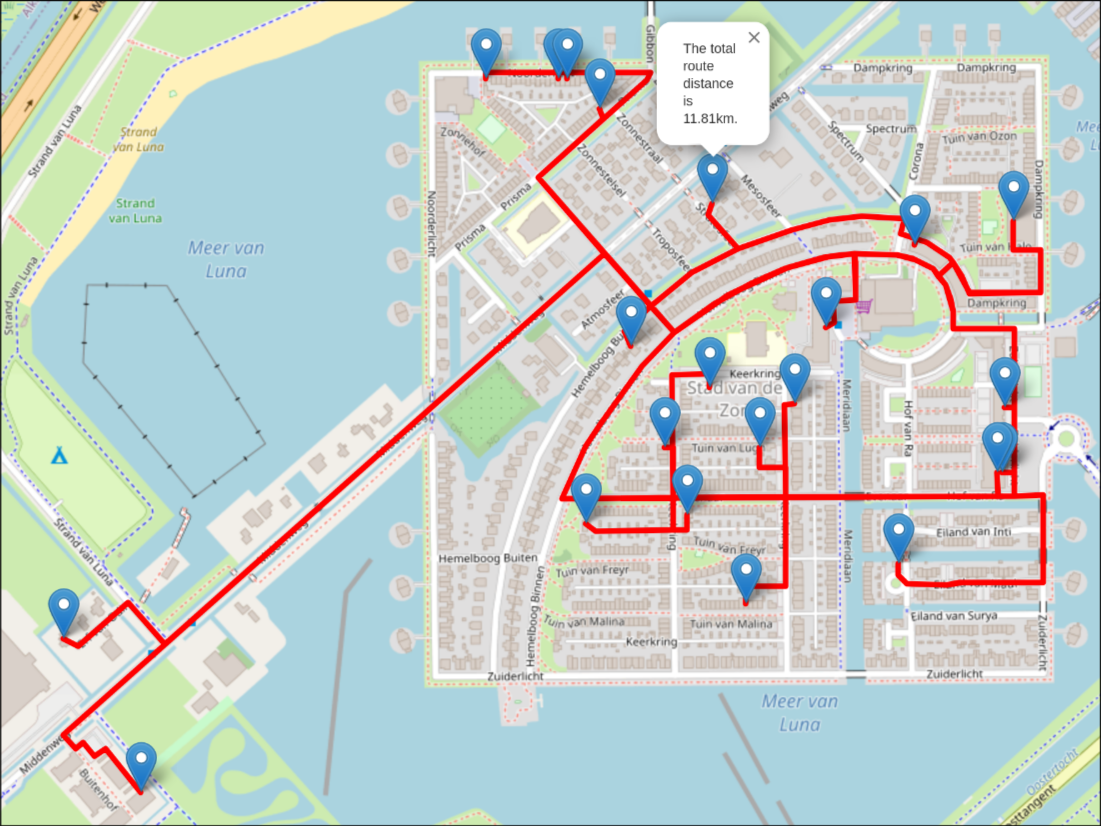
\includegraphics[width=\textwidth]{Pictures/TSP_22_Stad_van_de_Zon.png}
\end{figure}
